\subsection{ Body Sensor Network (BSN)}

A BSN foi criada para servir como um estudo de caso para o modelo arquitetural VerAACiTY \cite{caldasMestrado}, um modelo de verificação de sistemas auto-adaptativos dividido em camadas. A compreensão dessa arquitetura é fundamental para entender como o programa se organiza e interage.

A arquitetura da BSN, conforme ilustrado na Figura \ref{fig:arquitetura}, é composta por módulos principais, e o entendimento de cada um é vital para a compreensão do programa:

\begin{figure}[htb]
\centering
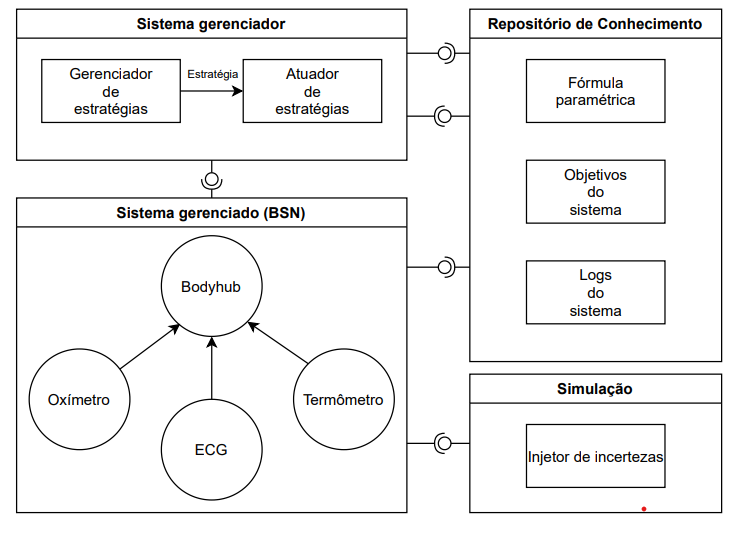
\includegraphics[width=.5\textwidth]{img/arquitetura.png}
\caption{Arquitetura da BSN \cite{Gil2021BodySN}}
\label{fig:arquitetura}
\end{figure}

\begin{itemize}
    \item \textbf{Sistema gerenciador}: Define e aplica estratégias de auto-adaptação com base na confiabilidade do sistema. Inclui o Strategy Manager, que estima confiabilidade e custo, e o Strategy Enactor, que ajusta a frequência dos componentes conforme as estratégias.

    \item \textbf{Sistema gerenciado}: É o próprio sistema da BSN, que coleta dados de sensores (termômetro, oxímetro, ECG) e os envia ao bodyhub (ou centralhub). O monitoramento ocorre via componentes probe (coleta) e param\_adapter (ação).

    \item \textbf{Repositório de conhecimento}: Armazena dados e fórmulas para o cálculo da confiabilidade, além dos objetivos do sistema e logs com informações sobre eventos, consumo e adaptação.

    \item \textbf{Simulação}: Injeta ruído nos sensores para simular falhas e testar a capacidade de adaptação do sistema em cenários com incerteza.
\end{itemize}
